\apendice{Documentación técnica de programación}
\label{apendice:documentacion_tecnica_programacion}
\label{apendice:programacion}

\section{Introducción}
\label{sec:d-introduccion}

Este anexo describe la organización técnica de los dos add-ons que forman la suite. A diferencia del anexo C, centrado en el diseño, aquí se explican las responsabilidades de los módulos, funciones, clases, dependencias, instalación, pruebas y pautas de mantenimiento.

La información se ordena de lo general a lo específico. Primero se presenta la estructura técnica del código, después el primer add-on de captura, a continuación el add-on de análisis y, finalmente, las tablas de funciones, dependencias, pruebas y criterios de mantenimiento.

\section{Estructura de directorios}
\label{sec:d-estructura-directorios}

La estructura técnica del proyecto se organiza en torno a los dos add-ons desarrollados. El primer add-on se distribuye como un único archivo Python, mientras que el segundo se organiza como un paquete modular con ficheros separados para el cálculo, la interfaz, la gestión de dependencias, las visualizaciones y las utilidades auxiliares.

\begin{verbatim}
codigo/
  DeteccionDatosV6.py
  analisisV7.zip

analisisV7/
  __init__.py
  analytics.py
  constants.py
  dependencies.py
  graphs.py
  operator.py
  ui.py
  ui_graph_rendering.py
  ui_graph_service.py
  ui_helpers.py
  ui_operators.py
  ui_panels.py
  ui_properties.py
  utils.py
  tests/
    test_logic.py
\end{verbatim}

\section{Primer add-on: \texttt{DeteccionDatosV6.py}}
\label{sec:d-logger}

\subsection{Variables globales}
\label{subsec:d-logger-globales}

El módulo emplea variables globales para mantener el estado mínimo necesario entre ciclos del temporizador. Entre ellas se encuentran el estado de ejecución del logger, el tiempo inicial de sesión, el último \textit{timestamp} registrado, los contadores topológicos previos, el modo anterior, el objeto activo anterior, la firma de snapshot previa, el hash UV anterior y las banderas de operadores. Este planteamiento evita almacenar un historial completo de la escena y permite calcular deltas de forma eficiente.

Las variables de depuración, como el último operador detectado, la última razón de registro o el estado del hash UV, se mantienen separadas del registro CSV. Su finalidad es facilitar la verificación durante el desarrollo y no sustituir los datos exportados.

\subsection{Gestión CSV}
\label{subsec:d-logger-csv}

La gestión CSV se concentra en funciones de inicialización, escritura incremental, restauración e incrustación. El archivo temporal se crea con una cabecera fija, se actualiza cuando se detectan cambios y se incrusta en el archivo \texttt{.blend} mediante un bloque de texto interno. Esta decisión reduce el riesgo de pérdida de datos cuando el usuario guarda el proyecto antes de exportar el CSV definitivo.

Las funciones principales de este bloque son \texttt{init\_csv}, \texttt{append\_csv}, \texttt{remove\_duplicate\_rows}, \texttt{import\_csv\_to\_blend} y \texttt{restore\_csv\_from\_blend}. La función \texttt{ensure\_file\_ends\_with\_newline} evita errores de concatenación al añadir filas sucesivas.

\subsection{Captura espacial}
\label{subsec:d-logger-espacial}

La captura espacial obtiene la posición de la vista 3D, el radio de escena y la posición/radio del objeto activo. Para ello se consultan áreas \texttt{VIEW\_3D}, matrices de vista y cajas envolventes transformadas a coordenadas de mundo. Este bloque proporciona los campos \texttt{UserX}, \texttt{UserY}, \texttt{UserZ}, \texttt{SceneRadius}, \texttt{ObjX}, \texttt{ObjY}, \texttt{ObjZ} y \texttt{ObjRadius}.

\subsection{Captura topológica}
\label{subsec:d-logger-topologica}

La captura topológica calcula el número de vértices, triángulos, n-gons y normales potencialmente invertidas. En \textit{Edit Mode} se utiliza \texttt{bmesh.from\_edit\_mesh} para acceder al estado editable de la malla; en \textit{Object Mode} se consulta directamente \texttt{obj.data}. La función \texttt{get\_mesh\_stats} centraliza esta lógica y devuelve una tupla con los contadores relevantes.

\subsection{Detección de operadores}
\label{subsec:d-logger-operadores}

La detección de operadores se basa en la normalización de identificadores de Blender y en banderas temporales. Se detectan operaciones de pegado, duplicación normal, duplicación enlazada y fusión o disolución. El operador \texttt{VIEW3D\_OT\_paste\_logger} encapsula \texttt{Ctrl+V} para conservar el comportamiento de pegado y registrar el evento de forma explícita.

\subsection{Detección UV}
\label{subsec:d-logger-uv}

La detección UV combina dos mecanismos. En primer lugar, se identifican operadores UV conocidos, como despliegue, empaquetado o proyección. En segundo lugar, se calcula un hash global de coordenadas UV mediante \texttt{get\_global\_uv\_hash}. Si el hash cambia respecto al estado anterior, el sistema marca un evento UV aunque no se haya producido una variación topológica.

\subsection{Snapshots y deltas}
\label{subsec:d-logger-snapshots}

El snapshot resume la escena en una estructura compacta: posición de usuario, radio de escena, objeto activo, contadores topológicos, modo, hash UV, número de objetos, número de modificadores y estado de oclusión. La función \texttt{build\_snapshot} construye esta representación y genera una firma comparable. La función \texttt{apply\_snapshot\_as\_baseline} actualiza la línea base cuando el estado se registra correctamente.

\subsection{Temporizador}
\label{subsec:d-logger-temporizador}

El temporizador se registra mediante \texttt{bpy.app.timers.register}. La función \texttt{logger\_timer} ejecuta la captura cada intervalo configurado mientras el logger está activo. Si existe una bandera de registro forzado, se escribe una fila aunque el cambio no haya sido detectado por la comparación ordinaria.

\subsection{Consentimiento}
\label{subsec:d-logger-consentimiento}

El consentimiento se implementa mediante un bloque de texto interno llamado \texttt{consent\_flag}. Si el usuario acepta, el texto almacena el valor \texttt{ACCEPTED}. El add-on también comprueba la configuración Auto Run de Blender y muestra un aviso cuando la ejecución automática de scripts está desactivada.

\subsection{Paneles}
\label{subsec:d-logger-paneles}

El add-on define un panel principal y un panel de depuración. El panel principal permite iniciar o detener el logger y exportar el CSV. El panel de depuración muestra estado del temporizador, último operador, motivo del último registro, estado UV y objeto activo. Este panel se mantiene cerrado por defecto para no saturar la interfaz.


\begin{figure}[H]
    \centering
    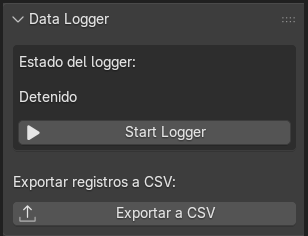
\includegraphics[width=0.65\textwidth]{diagramas/data_logger_sin_debug.png}
    \caption{Panel de depuración del add-on Data Logger 3D durante una sesión de captura.}
    \label{fig:d-panel-debug-logger}
\end{figure}

\begin{figure}[H]
    \centering
    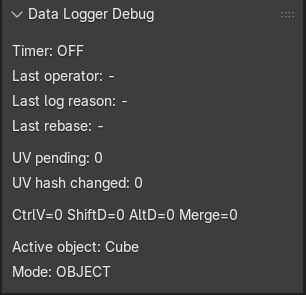
\includegraphics[width=0.65\textwidth]{diagramas/data_logger_con_debug.png}
    \caption{Panel de depuración del add-on Data Logger 3D durante una sesión de captura.}
    \label{fig:d-panel-debug-logger}
\end{figure}


\subsection{Exportación}
\label{subsec:d-logger-exportacion}

La exportación se realiza mediante \texttt{DATA\_LOGGER\_OT\_ExportCSV}. El operador comprueba que el archivo \texttt{.blend} esté guardado, que exista el bloque \texttt{data\_log\_internal.csv} y que su contenido no esté vacío. El CSV exportado se guarda en la misma carpeta que el \texttt{.blend}, con un nombre derivado del proyecto.

\subsection{Registro del add-on}
\label{subsec:d-logger-registro}

Las clases del add-on se registran mediante \texttt{bpy.utils.register\_class}. Además, se añaden keymaps, manejadores \texttt{load\_post}, \texttt{save\_post} y \texttt{depsgraph\_update\_post}. En \texttt{unregister} se eliminan keymaps y manejadores para evitar duplicados al recargar el script.

\section{Segundo add-on: análisis y visualización}
\label{sec:d-analisis}

\subsection{Lectura CSV}
\label{subsec:d-analisis-lectura}

La lectura de CSV se concentra en la capa de operadores e interfaz. El usuario puede seleccionar archivos o carpetas, y el sistema transforma los registros en estructuras utilizadas por \texttt{analytics.py}. El módulo acepta nombres de columnas esperados y variantes razonables en algunos campos temporales o espaciales.

\subsection{Validación}
\label{subsec:d-analisis-validacion}

La validación descarta valores no numéricos cuando no pueden convertirse, ignora valores no finitos y aplica funciones seguras como \texttt{safe\_float}, \texttt{series\_to\_array} y \texttt{clamp\_outliers}. Este proceso permite que una fila incompleta no detenga necesariamente todo el análisis, aunque los errores deben quedar visibles para depuración cuando proceda.

\subsection{Métricas A1--A17}
\label{subsec:d-analisis-a1-a17}

El módulo \texttt{analytics.py} define el diccionario \texttt{ANALYSIS} con las etiquetas y tipologías de A1--A17. La función \texttt{compute\_metrics\_for\_csv} calcula las métricas a partir de tiempos, posiciones de vista, posiciones de objeto, deltas, estados de modo y eventos. Las métricas se devuelven en un diccionario indexado por identificador, lo que facilita su presentación posterior.

\subsection{Métricas UV}
\label{subsec:d-analisis-uv}

Las métricas UV se implementan principalmente en \texttt{utils.py}. Incluyen conteo de islas UV, área UV, estiramiento y densidad de texeles. Estas funciones trabajan con capas UV activas y deben contemplar el caso de mallas sin coordenadas UV.

\subsection{Métricas geométricas}
\label{subsec:d-analisis-geometricas}

Las métricas geométricas se calculan sobre objetos de tipo malla. Incluyen similitud topológica, distancia de Hausdorff, duplicados de vértices, proporción de caras no cuadrangulares y comparación frente a referencia. Cuando se requiere comparar conjuntos de coordenadas, el cálculo debe controlar el tamaño de la malla para evitar tiempos excesivos.

\subsection{Métricas de normales}
\label{subsec:d-analisis-normales}

Las funciones \texttt{normal\_flipped} y \texttt{calculate\_normal\_percentage} evalúan la orientación de caras y calculan el porcentaje de normales potencialmente invertidas. Estas métricas ayudan a detectar problemas de calidad geométrica relevantes para modelos 3D.

\subsection{Métricas de ángulos}
\label{subsec:d-analisis-angulos}

La función \texttt{calculate\_angle\_median} resume los ángulos entre caras adyacentes. La mediana se utiliza para reducir el impacto de valores extremos y ofrecer una medida robusta del comportamiento angular de la malla.

\subsection{Visualización}
\label{subsec:d-analisis-visualizacion}

El módulo \texttt{graphs.py} genera gráficos y objetos de visualización dentro de Blender. Incluye funciones para limpiar visualizaciones previas, crear ejes, etiquetas, puntos, superficies, gráficos temporales, radar y comparativas multi-CSV. También se contemplan gráficos renderizados en memoria para evitar archivos intermedios cuando resulta posible.

\begin{figure}[H]
    \centering
    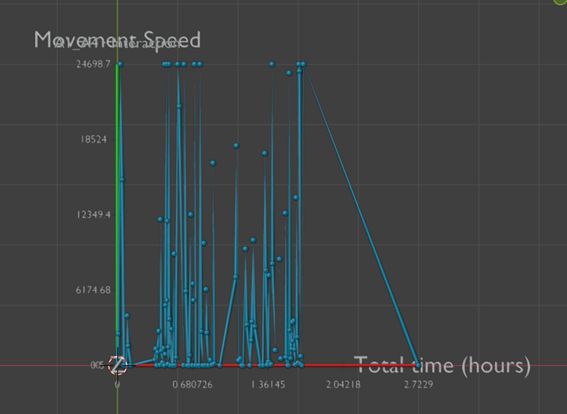
\includegraphics[width=0.85\textwidth]{diagramas/grafico1.png}
    \caption{Ejemplo de visualización generada por el add-on de análisis dentro de la escena de Blender.}
    \label{fig:d-visualizacion-blender}
\end{figure}

\subsection{Interfaz}
\label{subsec:d-analisis-interfaz}

La interfaz se distribuye en módulos \texttt{ui\_*}. Las propiedades se definen en \texttt{ui\_properties.py}, los paneles en \texttt{ui\_panels.py}, los operadores de interfaz en \texttt{ui\_operators.py} y las ayudas de presentación en \texttt{ui\_helpers.py}. Esta separación evita que el cálculo de métricas dependa directamente de los paneles.

\subsection{Registro del add-on}
\label{subsec:d-analisis-registro}

El registro se coordina desde \texttt{\_\_init\_\_.py} y \texttt{ui.py}. Cada módulo registra sus clases de Blender y expone las funciones necesarias para recargar el add-on. La estructura modular facilita desactivar o modificar paneles sin alterar la lógica de cálculo.


\section{Tabla completa de funciones}
\label{sec:d-tabla-funciones}

Las siguientes tablas agrupan las funciones y clases relevantes por módulo. Para mejorar la legibilidad, la información se divide en tres tablas independientes y se presenta en páginas apaisadas. De este modo se evita que las columnas queden comprimidas o que los nombres largos de funciones se salgan del margen.

\clearpage
{\pagestyle{empty}\thispagestyle{empty}
\begin{landscape}
\begingroup
\scriptsize
\setlength{\tabcolsep}{3pt}
\renewcommand{\arraystretch}{1.18}
\begin{longtable}{p{4.7cm}p{3.2cm}p{8.5cm}p{3.8cm}p{3.8cm}}
\caption{Funciones y clases principales del add-on Data Logger 3D.}\label{tab:d-funciones-logger}\\
\toprule
\textbf{Función / Clase} & \textbf{Módulo} & \textbf{Responsabilidad} & \textbf{Entrada principal} & \textbf{Salida principal} \\
\midrule
\endfirsthead
\caption[]{Funciones y clases principales del add-on Data Logger 3D (continuación).}\\
\toprule
\textbf{Función / Clase} & \textbf{Módulo} & \textbf{Responsabilidad} & \textbf{Entrada principal} & \textbf{Salida principal} \\
\midrule
\endhead
\midrule
\multicolumn{5}{r}{\textit{Continúa en la página siguiente}}\\
\endfoot
\bottomrule
\endlastfoot
\texttt{init\_csv} & \texttt{DeteccionDatosV6.py} & Crea el CSV temporal con la cabecera definida para la sesión de captura. & Ruta temporal global. & Archivo CSV inicializado. \\
\texttt{append\_csv} & \texttt{DeteccionDatosV6.py} & Añade una fila serializada al CSV, conservando el formato de salto de línea. & Fila CSV serializada. & CSV actualizado. \\
\texttt{ensure\_file\_ends\_with\_newline} & \texttt{DeteccionDatosV6.py} & Comprueba que el archivo termina con salto de línea para evitar concatenaciones erróneas entre filas. & Ruta del archivo CSV. & Archivo normalizado. \\
\texttt{remove\_duplicate\_rows} & \texttt{DeteccionDatosV6.py} & Elimina filas duplicadas manteniendo la cabecera original del CSV. & CSV temporal. & CSV sin duplicados. \\
\texttt{import\_csv\_to\_blend} & \texttt{DeteccionDatosV6.py} & Incrusta el contenido del CSV en un bloque de texto interno del archivo \texttt{.blend}. & CSV temporal. & \texttt{data\_log\_internal.csv}. \\
\texttt{restore\_csv\_from\_blend} & \texttt{DeteccionDatosV6.py} & Reconstruye el CSV temporal a partir del bloque de texto incrustado en Blender. & Bloque de texto interno. & CSV temporal reconstruido. \\
\texttt{get\_camera\_pos} & \texttt{DeteccionDatosV6.py} & Obtiene la posición de la vista 3D activa mediante la matriz de vista. & Contexto de Blender. & Coordenadas \texttt{UserX}, \texttt{UserY}, \texttt{UserZ}. \\
\texttt{get\_active\_object\_data} & \texttt{DeteccionDatosV6.py} & Calcula centro y radio del objeto activo a partir de su caja envolvente en coordenadas de mundo. & Objeto activo. & Tupla espacial del objeto. \\
\texttt{get\_scene\_radius} & \texttt{DeteccionDatosV6.py} & Estima el radio global de la escena considerando las cajas envolventes de las mallas. & Objetos de la escena. & Radio de escena. \\
\texttt{get\_mesh\_stats} & \texttt{DeteccionDatosV6.py} & Calcula contadores topológicos de vértices, triángulos, n-gons y normales potencialmente invertidas. & Objeto malla. & Contadores topológicos. \\
\texttt{get\_global\_uv\_hash} & \texttt{DeteccionDatosV6.py} & Resume las coordenadas UV de la escena mediante un hash para detectar cambios. & Escena y capas UV. & Cadena hash. \\
\texttt{detect\_flags\_from\_operator} & \texttt{DeteccionDatosV6.py} & Activa banderas de operadores como \texttt{Ctrl+V}, \texttt{Shift+D}, \texttt{Alt+D}, \texttt{Merge} y operaciones UV. & Identificador de operador. & Booleano de cambio. \\
\texttt{process\_new\_operators} & \texttt{DeteccionDatosV6.py} & Recorre los operadores recientes registrados por Blender y actualiza las banderas pendientes. & Historial de operadores. & Indicador de cambio. \\
\texttt{build\_snapshot} & \texttt{DeteccionDatosV6.py} & Construye un resumen del estado de la escena y una firma comparable entre ciclos. & Contexto de Blender. & Snapshot y firma. \\
\texttt{apply\_snapshot\_as\_baseline} & \texttt{DeteccionDatosV6.py} & Actualiza el estado de referencia usado para calcular deltas posteriores. & Snapshot y firma. & Línea base actualizada. \\
\texttt{collect\_data} & \texttt{DeteccionDatosV6.py} & Calcula deltas, estados de modo, banderas de operador y genera una fila CSV cuando hay cambios. & Estado actual de la escena. & Fila CSV o \texttt{None}. \\
\texttt{logger\_timer} & \texttt{DeteccionDatosV6.py} & Ejecuta ciclos periódicos de captura mediante el temporizador de Blender. & Temporizador de Blender. & Intervalo de repetición o \texttt{None}. \\
\texttt{DATA\_LOGGER\_OT\_ExportCSV} & \texttt{DeteccionDatosV6.py} & Exporta el CSV incrustado a un archivo externo junto al archivo \texttt{.blend}. & Contexto de Blender. & Archivo CSV exportado. \\
\texttt{DATA\_LOGGER\_PT\_Panel} & \texttt{DeteccionDatosV6.py} & Muestra el panel principal de control del logger en la barra lateral de Blender. & Contexto de interfaz. & Panel de usuario. \\
\texttt{DATA\_LOGGER\_PT\_DebugPanel} & \texttt{DeteccionDatosV6.py} & Muestra información de depuración sobre operadores, hash UV y estado del temporizador. & Contexto de interfaz. & Panel de depuración. \\
\texttt{register}/\texttt{unregister} & \texttt{DeteccionDatosV6.py} & Registra o elimina clases, keymaps y handlers del add-on. & Runtime de Blender. & Add-on activo o inactivo. \\
\end{longtable}
\endgroup
\end{landscape}

\clearpage
{\pagestyle{empty}\thispagestyle{empty}
\begin{landscape}
\begingroup
\scriptsize
\setlength{\tabcolsep}{3pt}
\renewcommand{\arraystretch}{1.18}
\begin{longtable}{p{4.7cm}p{3.2cm}p{8.5cm}p{3.8cm}p{3.8cm}}
\caption{Funciones principales de cálculo y validación del add-on de análisis.}\label{tab:d-funciones-analisis}\\
\toprule
\textbf{Función / Clase} & \textbf{Módulo} & \textbf{Responsabilidad} & \textbf{Entrada principal} & \textbf{Salida principal} \\
\midrule
\endfirsthead
\caption[]{Funciones principales de cálculo y validación del add-on de análisis (continuación).}\\
\toprule
\textbf{Función / Clase} & \textbf{Módulo} & \textbf{Responsabilidad} & \textbf{Entrada principal} & \textbf{Salida principal} \\
\midrule
\endhead
\midrule
\multicolumn{5}{r}{\textit{Continúa en la página siguiente}}\\
\endfoot
\bottomrule
\endlastfoot
\texttt{safe\_float} & \texttt{analytics.py} & Convierte campos CSV a número de forma segura y evita errores por valores no numéricos. & Fila y clave. & Valor flotante. \\
\texttt{series\_to\_array} & \texttt{analytics.py} & Limpia series numéricas y descarta valores no finitos antes del cálculo estadístico. & Secuencia de valores. & \texttt{ndarray}. \\
\texttt{clamp\_outliers} & \texttt{analytics.py} & Limita valores extremos mediante el rango intercuartílico. & Serie numérica. & Serie acotada. \\
\texttt{compute\_metrics\_for\_csv} & \texttt{analytics.py} & Calcula las métricas A1--A17 a partir de las filas validadas del CSV. & Filas CSV. & Diccionario de métricas. \\
\texttt{ensure\_modules} & \texttt{dependencies.py} & Comprueba la disponibilidad de dependencias externas necesarias para el análisis. & Lista de módulos. & Estado de disponibilidad. \\
\texttt{count\_uv\_islands} & \texttt{utils.py} & Cuenta islas UV a partir de la conectividad de la malla y sus coordenadas UV. & \texttt{bmesh}. & Número de islas UV. \\
\texttt{calculate\_uv\_area} & \texttt{utils.py} & Calcula el área ocupada por las coordenadas UV de la malla. & Malla y capa UV. & Área UV. \\
\texttt{calculate\_uv\_stretch} & \texttt{utils.py} & Estima la relación de estiramiento entre geometría 3D y despliegue UV. & Objeto malla. & Valor de stretch. \\
\texttt{calculate\_uv\_texel\_density} & \texttt{utils.py} & Calcula una medida de densidad de texeles asociada al despliegue UV. & Objeto malla. & Densidad. \\
\texttt{calculate\_normal\_percentage} & \texttt{utils.py} & Calcula el porcentaje de normales anómalas o invertidas respecto al total evaluado. & Objeto o \texttt{BMesh}. & Porcentaje. \\
\texttt{calculate\_angle\_median} & \texttt{utils.py} & Resume mediante la mediana los ángulos entre caras adyacentes. & \texttt{bmesh}. & Mediana angular. \\
\texttt{calculate\_similarity} & \texttt{utils.py} & Compara un objeto analizado con una referencia para estimar su similitud geométrica. & Dos objetos. & Porcentaje o puntuación. \\
\shortstack[l]{\texttt{calculate\_hausdorff}\\\texttt{\_distance\_from\_coords}} & \texttt{utils.py} & Calcula la distancia de Hausdorff entre dos conjuntos de coordenadas. & Dos conjuntos de coordenadas. & Distancia. \\
\end{longtable}
\endgroup
\end{landscape}

\clearpage
{\pagestyle{empty}\thispagestyle{empty}
\begin{landscape}
\begingroup
\scriptsize
\setlength{\tabcolsep}{3pt}
\renewcommand{\arraystretch}{1.18}
\begin{longtable}{p{4.7cm}p{3.2cm}p{8.5cm}p{3.8cm}p{3.8cm}}
\caption{Funciones y grupos de interfaz/visualización del add-on de análisis.}\label{tab:d-funciones-ui}\\
\toprule
\textbf{Función / Clase} & \textbf{Módulo} & \textbf{Responsabilidad} & \textbf{Entrada principal} & \textbf{Salida principal} \\
\midrule
\endfirsthead
\caption[]{Funciones y grupos de interfaz/visualización del add-on de análisis (continuación).}\\
\toprule
\textbf{Función / Clase} & \textbf{Módulo} & \textbf{Responsabilidad} & \textbf{Entrada principal} & \textbf{Salida principal} \\
\midrule
\endhead
\midrule
\multicolumn{5}{r}{\textit{Continúa en la página siguiente}}\\
\endfoot
\bottomrule
\endlastfoot
\texttt{clear\_previous\_graphs} & \texttt{graphs.py} & Elimina visualizaciones anteriores para evitar solapamientos en la escena. & Escena. & Escena limpia. \\
\texttt{create\_axis} & \texttt{graphs.py} & Crea ejes de referencia para representar métricas en el espacio 3D. & Coordenadas y escala. & Objeto eje. \\
\texttt{create\_text\_label} & \texttt{graphs.py} & Genera etiquetas de texto asociadas a gráficos y valores. & Texto y posición. & Objeto de texto. \\
\texttt{draw\_metric\_line} & \texttt{graphs.py} & Dibuja una línea asociada a la evolución de una métrica. & Serie métrica. & Curva u objeto gráfico. \\
\texttt{create\_time\_graph} & \texttt{graphs.py} & Genera un gráfico temporal a partir de una serie o un CSV. & CSV o serie. & Visualización temporal. \\
\texttt{draw\_surface\_graph} & \texttt{graphs.py} & Construye una superficie gráfica a partir de valores X, Y y Z. & Valores X/Y/Z. & Objeto superficie. \\
\shortstack[l]{\texttt{draw\_multi\_csv}\\\texttt{\_forest\_plot\_3d}} & \texttt{graphs.py} & Compara varios CSV mediante una representación tridimensional tipo forest plot. & Conjunto de CSV. & Forest plot 3D. \\
\shortstack[l]{\texttt{draw\_radar\_graph}\\\texttt{\_3d\_filled}} & \texttt{graphs.py} & Genera un gráfico radar 3D con métricas normalizadas. & Métricas normalizadas. & Objeto radar. \\
\texttt{ui\_panels} & \texttt{ui\_panels.py} & Define los paneles de resultados y la disposición visual de los bloques de métricas. & Contexto de Blender. & Panel de interfaz. \\
\texttt{ui\_operators} & \texttt{ui\_operators.py} & Ejecuta acciones desde botones de la interfaz, como carga de CSV o cálculo de métricas. & Contexto y propiedades. & Resultado de operador. \\
\texttt{ui\_properties} & \texttt{ui\_properties.py} & Define propiedades configurables y rutas utilizadas por la interfaz. & Escena o \texttt{WindowManager}. & Propiedades registradas. \\
\texttt{register}/\texttt{unregister} & \texttt{\_\_init\_\_.py} & Registra o elimina las clases y módulos del add-on de análisis. & Runtime de Blender. & Add-on activo o inactivo. \\
\end{longtable}
\endgroup
\end{landscape}
}

\clearpage
\section{Compilación, instalación y ejecución}
\label{sec:d-instalacion-ejecucion}

Para instalar el primer add-on se debe utilizar el archivo \texttt{DeteccionDatosV6.py} desde las preferencias de Blender. Para instalar el segundo add-on se debe utilizar el ZIP del paquete de análisis. En ambos casos, el flujo general es: abrir Blender, acceder a \textit{Edit $\rightarrow$ Preferences $\rightarrow$ Add-ons}, instalar el archivo correspondiente, activar la casilla del add-on y guardar preferencias si se desea conservar la activación.

La ejecución completa comienza con el add-on de captura, continúa con la exportación del CSV y finaliza con la lectura del CSV desde el add-on de análisis. Las pruebas que dependan de paneles, operadores o mallas reales deben realizarse dentro de Blender.

\section{Dependencias externas}
\label{sec:d-dependencias}

Las dependencias principales son Blender, Python integrado en Blender, \texttt{bpy}, \texttt{bmesh}, \texttt{mathutils}, \texttt{csv}, NumPy y Matplotlib. El logger depende principalmente de la API de Blender y de módulos estándar de Python. El add-on de análisis incorpora dependencias científicas para el cálculo de métricas y la representación gráfica de resultados.

La versión desarrollada se ha probado sobre un entorno basado en Python 3.11, integrado en versiones recientes de Blender. Por este motivo, no se garantiza la compatibilidad con Blender 3.0 ni con versiones anteriores que utilicen intérpretes de Python más antiguos o APIs parcialmente diferentes. La retrocompatibilidad con dichas versiones requeriría revisar las llamadas a la API de Blender, las dependencias científicas y los módulos utilizados por el add-on de análisis.

En consecuencia, se recomienda utilizar la suite en versiones de Blender compatibles con Python 3.11. Las versiones consideradas compatibles en el entorno de desarrollo son Blender 4.0 y posteriores, hasta la versión 5.1.2. Para versiones futuras, será necesario verificar que no se hayan producido cambios incompatibles en la API de Blender o en la gestión de add-ons.

\section{Pruebas del sistema}
\label{sec:d-pruebas}

Las pruebas se ordenan por nivel. En el logger se deben comprobar inicio/parada, consentimiento, restauración del CSV, exportación, captura de cambios de modo, detección de operadores, cambios UV y persistencia en \texttt{.blend}. En el add-on de análisis se deben comprobar lectura CSV, rechazo de valores NaN o infinitos, cálculo A1--A17, cálculo geométrico, métricas UV, generación de visualizaciones e interfaz compacta.

Las pruebas fuera de Blender son limitadas para funciones que dependen de \texttt{bpy}, paneles o contexto gráfico. No obstante, parte de la lógica analítica puede probarse con datos CSV simulados o con pruebas unitarias sobre funciones puras.

\section{Mantenimiento y ampliación}
\label{sec:d-mantenimiento}

El mantenimiento de la suite requiere conservar la coherencia entre el logger, el formato CSV y el add-on de análisis. Si se añaden nuevos campos al CSV, deben actualizarse la cabecera, la construcción de registros y la validación de lectura en el módulo de análisis. Del mismo modo, cualquier nueva métrica debe incorporarse en la lógica de cálculo correspondiente, reflejarse en la interfaz y documentarse en el manual de usuario para facilitar su interpretación.

La ampliación del logger puede realizarse añadiendo nuevos operadores detectables al conjunto de identificadores normalizados y revisando si dichos eventos requieren un registro forzado. En el caso de nuevas visualizaciones, se recomienda mantener separada la lógica de cálculo respecto a la creación de objetos gráficos en Blender. Esta separación facilita la depuración, reduce dependencias entre módulos y permite ampliar la herramienta sin modificar de forma innecesaria el resto del sistema.